%package list
\documentclass{article}
\usepackage[top=3cm, bottom=3cm, outer=3cm, inner=3cm]{geometry}
\usepackage{multicol}
\usepackage{graphicx}
\usepackage{url}
%\usepackage{cite}
\usepackage{hyperref}
\usepackage{array}
%\usepackage{multicol}
\newcolumntype{x}[1]{>{\centering\arraybackslash\hspace{0pt}}p{#1}}
\usepackage{natbib}
\usepackage{pdfpages}
\usepackage{multirow}
\usepackage[normalem]{ulem}
\useunder{\uline}{\ul}{}
\usepackage{svg}
\usepackage{xcolor}
\usepackage{listings}
\lstdefinestyle{ascii-tree}{
	literate={├}{|}1 {─}{--}1 {└}{+}1 
}
\lstset{basicstyle=\ttfamily,
	showstringspaces=false,
	commentstyle=\color{red},
	keywordstyle=\color{blue}
}
%\usepackage{booktabs}
\usepackage{caption}
\usepackage{subcaption}
\usepackage{float}
\usepackage{array}

\newcolumntype{M}[1]{>{\centering\arraybackslash}m{#1}}
\newcolumntype{N}{@{}m{0pt}@{}}


%%%%%%%%%%%%%%%%%%%%%%%%%%%%%%%%%%%%%%%%%%%%%%%%%%%%%%%%%%%%%%%%%%%%%%%%%%%%
%%%%%%%%%%%%%%%%%%%%%%%%%%%%%%%%%%%%%%%%%%%%%%%%%%%%%%%%%%%%%%%%%%%%%%%%%%%%
\newcommand{\itemEmail}{jchuraaca@unsa.edu.pe}
\newcommand{\itemStudent}{Julio Rubén Chura Acabana}
\newcommand{\itemCourse}{ F. de Programción 2}
\newcommand{\itemCourseCode}{20230472}
\newcommand{\itemSemester}{I}
\newcommand{\itemUniversity}{Universidad Nacional de San Agustín de Arequipa}
\newcommand{\itemFaculty}{Facultad de Ingeniería de Producción y Servicios}
\newcommand{\itemDepartment}{Departamento Académico de Ingeniería de Sistemas e Informática}
\newcommand{\itemSchool}{Escuela Profesional de Ingeniería de Sistemas}
\newcommand{\itemAcademic}{2023 - B}
\newcommand{\itemInput}{Del 20 Septiembre 2023}
\newcommand{\itemOutput}{Al 25 Septiembre 2023}
\newcommand{\itemPracticeNumber}{04}
\newcommand{\itemTheme}{Arreglos de Objetos, Búsqueda y Ordenamiento de Burbuja}
%%%%%%%%%%%%%%%%%%%%%%%%%%%%%%%%%%%%%%%%%%%%%%%%%%%%%%%%%%%%%%%%%%%%%%%%%%%%
%%%%%%%%%%%%%%%%%%%%%%%%%%%%%%%%%%%%%%%%%%%%%%%%%%%%%%%%%%%%%%%%%%%%%%%%%%%%

\usepackage[english,spanish]{babel}
\usepackage[utf8]{inputenc}
\AtBeginDocument{\selectlanguage{spanish}}
\renewcommand{\figurename}{Figura}
\renewcommand{\refname}{Referencias}
\renewcommand{\tablename}{Tabla} %esto no funciona cuando se usa babel
\AtBeginDocument{%
	\renewcommand\tablename{Tabla}
}

\usepackage{fancyhdr}
\pagestyle{fancy}
\fancyhf{}
\setlength{\headheight}{30pt}
\renewcommand{\headrulewidth}{1pt}
\renewcommand{\footrulewidth}{1pt}
\fancyhead[L]{\raisebox{-0.2\height}{
\includegraphics[width=3cm]{img/logo_episunsa.png}}}
\fancyhead[C]{\fontsize{7}{7}\selectfont	\itemUniversity \\ \itemFaculty \\ \itemDepartment \\ \itemSchool \\ \textbf{\itemCourse}}
\fancyhead[R]{\raisebox{-0.2\height}{
\includegraphics[width=1.2cm]{img/logo_abet}}}
\fancyfoot[L]{Estudiante Julio Rubén Chura Acabana}
\fancyfoot[C]{\itemCourse}
\fancyfoot[R]{Página \thepage}

% para el codigo fuente
\usepackage{listings}
\usepackage{color, colortbl}
\definecolor{dkgreen}{rgb}{0,0.6,0}
\definecolor{gray}{rgb}{0.5,0.5,0.5}
\definecolor{mauve}{rgb}{0.58,0,0.82}
\definecolor{codebackground}{rgb}{0.95, 0.95, 0.92}
\definecolor{tablebackground}{rgb}{0.8, 0, 0}

\lstset{frame=tb,
	language=bash,
	aboveskip=3mm,
	belowskip=3mm,
	showstringspaces=false,
	columns=flexible,
	basicstyle={\small\ttfamily},
	numbers=none,
	numberstyle=\tiny\color{gray},
	keywordstyle=\color{blue},
	commentstyle=\color{dkgreen},
	stringstyle=\color{mauve},
	breaklines=true,
	breakatwhitespace=true,
	tabsize=3,
	backgroundcolor= \color{codebackground},
}

\begin{document}
	
	\vspace*{10px}
	
	\begin{center}	
		\fontsize{17}{17} \textbf{ Informe de Laboratorio \itemPracticeNumber}
	\end{center}
	\centerline{\textbf{\Large Tema: \itemTheme}}
	%\vspace*{0.5cm}	
	
	\begin{flushright}
		\begin{tabular}{|M{2.5cm}|N|}
			\hline 
			\rowcolor{tablebackground}
			\color{white} \textbf{Nota}  \\
			\hline 
			\\[30pt]
			\hline 			
		\end{tabular}
	\end{flushright}	
	
	\begin{table}[H]
		\begin{tabular}{|x{4.7cm}|x{4.8cm}|x{4.8cm}|}
			\hline 
			\rowcolor{tablebackground}
			\color{white} \textbf{Estudiante} & \color{white}\textbf{Escuela}  & \color{white}\textbf{Asignatura}   \\
			\hline 
			{\itemStudent \par \itemEmail} & \itemSchool & {\itemCourse \par Semestre: \itemSemester \par Código: \itemCourseCode}     \\
			\hline 			
		\end{tabular}
	\end{table}		
	
	\begin{table}[H]
		\begin{tabular}{|x{4.7cm}|x{4.8cm}|x{4.8cm}|}
			\hline 
			\rowcolor{tablebackground}
			\color{white}\textbf{Laboratorio} & \color{white}\textbf{Tema}  & \color{white}\textbf{Duración}   \\
			\hline 
			\itemPracticeNumber & \itemTheme & 04 horas   \\
			\hline 
		\end{tabular}
	\end{table}
	
	\begin{table}[H]
		\begin{tabular}{|x{4.7cm}|x{4.8cm}|x{4.8cm}|}
			\hline 
			\rowcolor{tablebackground}
			\color{white}\textbf{Semestre académico} & \color{white}\textbf{Fecha de inicio}  & \color{white}\textbf{Fecha de entrega}   \\
			\hline 
			\itemAcademic & \itemInput &  \itemOutput  \\
			\hline 
		\end{tabular}
	\end{table}
	
	\section{Tarea}
	\begin{itemize}		
		\item 
		En esta práctica se le dará un código incompleto donde deberá completar los métodos. Se le solicita utilizar los distintos tipos de búsqueda como la lineal y la binaria. También deberá hacer uso de los algoritmos de ordenamiento (Selección, inserción y burbuja)
		\item Usted debe realizar varios commits y al término de la actividad deberá elaborar un informe
		
	\end{itemize}
	
	\section{Equipos, materiales y temas utilizados}
	\begin{itemize}
		\item Sistema Operativo Windows
		\item VIM 9.0.
		\item OpenJDK 64-Bits 17.0.7.
		\item Git 2.39.2.
		\item Cuenta en GitHub con el correo institucional.
		\item Arreglos Estándar
	\end{itemize}
	
	\section{URL de Repositorio Github}
	\begin{itemize}
		\item URL del Repositorio GitHub para clonar o recuperar.
		\item \url{https://github.com/JulioChura/fp2-23b.git}
		\item URL para el laboratorio 01 en el Repositorio GitHub.
		\item \url{https://github.com/JulioChura/fp2-23b/tree/main/fase01/lab04}
	\end{itemize}
	
	\section{Actividades con el repositorio GitHub}
	

	
	\begin{lstlisting}[language=bash,caption={Preparando los archivos, para ello se copiará el código del lab03 al lab04 }][H]
		mkdir lab04
		cd lab01
		Copy-Item -Path "Nave.java" -Destination "..\lab04"
		Copy-Item -Path "DemoBatalla" -Destination "..\lab04"
		cd ..
		cd lab04	
		
		
	\end{lstlisting}
	
	\begin{lstlisting}[language=bash,caption={Se copian los métodos que faltan al código DemoBatalla.java, ahora solo hay que completar los métodos}][H]
		vim DemoBatalla.java
	\end{lstlisting}
	
		
	\begin{lstlisting}[language=bash,caption={Commit: Codigo de la practica de lab04 sin llenar los nuevos metodos }][H]
		git add DemoBatalla.java
		git commit -m "Codigo de la practica de lab04 sin llenar los nuevos metodos"
		git push -u origin main
	\end{lstlisting}
	
	
	
	\begin{lstlisting}[language=bash,caption={Implementado el método busquedaLinealNombre}][H]
		vim DemoBatalla.java
	\end{lstlisting}
	
	
	\begin{itemize}	
		\item El método se encarga de retornar el índice donde se encuentre la palabra solicitada por el usuario, en caso de no encontrar se retorna un -1. 
	\end{itemize}	
	
	\begin{figure}[H]
		\centering
		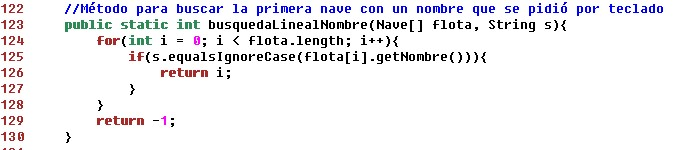
\includegraphics[width=1\textwidth,keepaspectratio]{img/2.jpg}
		%\includesvg{img/automata.svg}
		%\label{img:mot2}
		%\caption{Product backlog.}
	\end{figure}
	
		
	\begin{itemize}	
		\item Para ver el funcionamiento del método, se implementa en el main lo necesario. Lo más interesante son las condicionales, en caso el número sea -1, se imprime un mensaje de que no fue encontrada la nave, caso contrario se imprime todos los datos de esta.
	\end{itemize}	
	
	\begin{figure}[H]
		\centering
		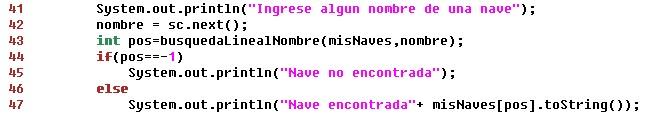
\includegraphics[width=1\textwidth,keepaspectratio]{img/1.jpg}
		%\includesvg{img/automata.svg}
		%\label{img:mot2}
		%\caption{Product backlog.}
	\end{figure}
		
	\begin{itemize}	
		\item Para poder probar el método, se cambio el tamaño del arreglo siendo ahora de 2, además que algunas líneas fueron puestas como comentarios para evitar que al momento de imprimir, sea algo extenso
	\end{itemize}
	
	\begin{lstlisting}[language=bash,caption={Probando el metodo busquedaLinealNombre}][H]	
		javac DemoBatalla.java
		java DemoBatalla.java
		Nave 1
		Nombre: alfa
		Fila
		3
		Columna: 5
		Estado: true
		Puntos: 43
		Nave 2
		Nombre: beta
		Fila
		43
		Columna: 5
		Estado: true
		Puntos: 43
		Ingrese algun nombre de una nave
		beta
		Nave encontradaNombre: beta, Fila: 43, Columna: 5, Estado; true, Puntos: 43
		
	\end{lstlisting}
	\begin{lstlisting}[language=bash,caption={Commit: Metodo busquedaLinealNombre completo}][H]
		git add DemoBatalla.java
		git commit -m "Metodo busquedaLinealNombre completo"			
		git push -u origin main
	\end{lstlisting}
	
	

	
	
	
	
	
	
	
	\begin{lstlisting}[language=bash,caption={Implementadno el método de ordenarPorPuntosBurbuja}][H]
		vim DemoBatalla.java
	\end{lstlisting}
	
	
	\begin{itemize}	
		\item En este método se pretende ordenar los puntos que tiene cada nave  usando el ordenamiento burbuja
	\end{itemize}	
	
	\begin{figure}[H]
		\centering
		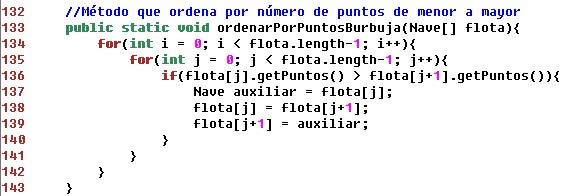
\includegraphics[width=1\textwidth,keepaspectratio]{img/3.jpg}
		%\includesvg{img/automata.svg}
		%\label{img:mot2}
		%\caption{Product backlog.}
	\end{figure}

	
	\begin{lstlisting}[language=bash,caption={Probando el metodo ordenarPorPuntosBurbuja}][H]	
		javac DemoBatalla.java
		java DemoBatalla.java
		Nave 1
		Nombre: alfa
		Fila
		34
		Columna: 5
		Estado: true
		Puntos: 34
		Nave 2
		Nombre: beta
		Fila
		43
		Columna: 5
		Estado: true
		Puntos: 6
		Nave 3
		Nombre: coraza
		Fila
		3
		Columna: 6
		Estado: true
		Puntos: 55
		Nave 1: Nombre: beta, Fila: 43, Columna: 5, Estado; true, Puntos: 6
		Nave 2: Nombre: alfa, Fila: 34, Columna: 5, Estado; true, Puntos: 34
		Nave 3: Nombre: coraza, Fila: 3, Columna: 6, Estado; true, Puntos: 55
		
	\end{lstlisting}
	\begin{lstlisting}[language=bash,caption={Commit: Metodo ordenarPorPuntosBurbuja fue culminado }][H]
		git add DemoBatalla.java
		git commit -m "Metodo ordenarPorPuntosBurbuja"			
		git push -u origin main
	\end{lstlisting}
	
	
	
	
	
	
	
	
	
	
	
	
	
	
	
	
	
	
	
	
	
	
	
	
	
	
	
	
	
	
	
	
	
	
	\begin{lstlisting}[language=bash,caption={Implementado el método ordenarPorNombreBurbuja}][H]
		vim DemoBatalla.java
	\end{lstlisting}
	
	
	\begin{itemize}	
		\item El método se encarga de ordenar de forma alfabética los Strings de un arreglo. Se hace uso del método compareTo(String s) el cual retorna un número negativo si s es mayor que el otro string, retorna un valor positivo cuando s es menor que el otro string y cero cuando ambos strings son iguales. Luego se sigue la misma lógica del ordenamiento Burbuja
	\end{itemize}	
	
	
	
	\begin{figure}[H]
		\centering
		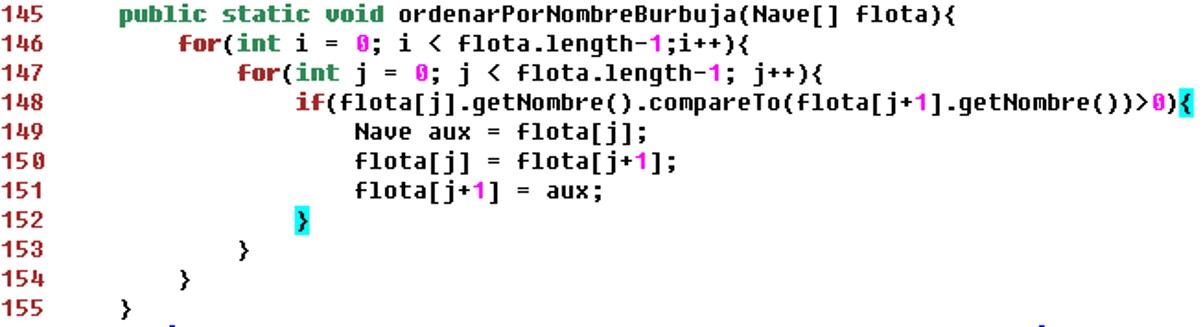
\includegraphics[width=1\textwidth,keepaspectratio]{img/4.jpg}
		%\includesvg{img/automata.svg}
		%\label{img:mot2}
		%\caption{Product backlog.}
	\end{figure}
	
	\begin{itemize}	
		\item Para poder probar el método, se cambio el tamaño del arreglo siendo ahora de 3, además que algunas líneas fueron puestas como comentarios para evitar que al momento de imprimir, sea algo extenso
	\end{itemize}
	
	\begin{lstlisting}[language=bash,caption={Probando el metodo ordenarPorNombreBurbuja}][H]	
		Nave 1
		Nombre: caza
		Fila
		5
		Columna: 6
		Estado: true
		Puntos: 34
		Nave 2
		Nombre: alfa
		Fila
		23
		Columna: 5
		Estado: true
		Puntos: 67
		Nave 3
		Nombre: alcon
		Fila
		3
		Columna: 6
		Estado: true
		Puntos: 87
		Nave 1: Nombre: alcon, Fila: 3, Columna: 6, Estado; true, Puntos: 87
		Nave 2: Nombre: alfa, Fila: 23, Columna: 5, Estado; true, Puntos: 67
		Nave 3: Nombre: caza, Fila: 5, Columna: 6, Estado; true, Puntos: 34
		
	\end{lstlisting}
	\begin{lstlisting}[language=bash,caption={Commit:"Método ordenarPorNombreBurbuja culminado" }][H]
		git add DemoBatalla.java
		git commit -m "Metodo ordenarPorNombreBurbuja culminado"			
		git push -u origin main
	\end{lstlisting}
	
	
	

	
	\begin{lstlisting}[language=bash,caption={Implementado el método busquedaBinariaNombre }][H]
		vim DemoBatalla.java
	\end{lstlisting}
	
	
	\begin{itemize}	
		\item El método se encarga de hacer la búsqueda de un string ingresado por el usuario. Se hace uso del algoritmo de búsqueda binaria. Se usa los métodos equals para determinar si el String en la posición media es igual al solicitado y también se hace uso del método compareTo para determinar las posiciones alta y baja para seguir con el flujo algoritmo. Si no se encuentran coincidencias, se retorna el valor de -1. Se añadieron líneas en el main para que el método reciba los parámetros y pueda hacer su búsqueda. Una vez el método retorne un valor de tipo entero, dicho valor será evaluado en una estructura condicional y de acuerdo a las condiciones se imprime un mensaje.
	\end{itemize}	
	
	\begin{figure}[H]
		\centering
		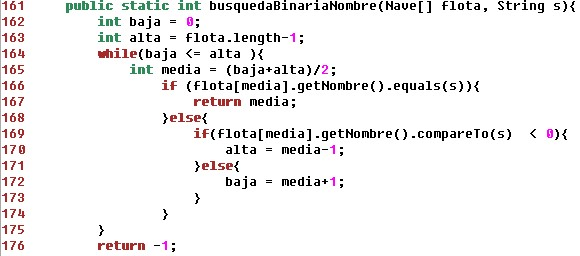
\includegraphics[width=0.9\textwidth,keepaspectratio]{img/7.jpg}
		%\includesvg{img/automata.svg}
		%\label{img:mot2}
		%\caption{Product backlog.}
	\end{figure}
	
	\begin{itemize}	
		\item Fragmento de código en el main
	\end{itemize}
	
	\begin{figure}[H]
		\centering
		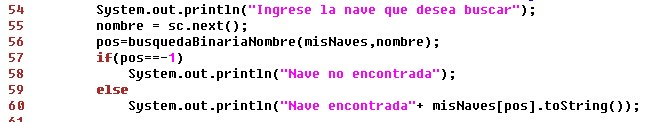
\includegraphics[width=1.1\textwidth,keepaspectratio]{img/8.jpg}
		%\includesvg{img/automata.svg}
		%\label{img:mot2}
		%\caption{Product backlog.}
	\end{figure}
	
	
	\begin{lstlisting}[language=bash,caption={Probando el metodo busquedaBinariaNombre}][H]	
		javac DemoBatalla.java
		java DemoBatalla
		Nave 1
		Nombre: alfa
		Fila
		5
		Columna: 6
		Estado: true
		Puntos: 34
		Nave 2
		Nombre: beta
		Fila
		3
		Columna: 4
		Estado: true
		Puntos: 8
		Nave 3
		Nombre: gama
		Fila
		3
		Columna: 4
		Estado: true
		Puntos: 32
		Ingrese la nave que desea buscar
		beta
		Nave encontradaNombre: beta, Fila: 3, Columna: 4, Estado; true, Puntos: 8
	\end{lstlisting}
	\begin{lstlisting}[language=bash,caption={Commit:"Metodo busquedaBinariaNombre" }][H]
		git add DemoBatalla.java
		git commit -m "Metodo busquedaBinariaNombre"			
		git push -u origin main
	\end{lstlisting}
	
	
	
	
	

	
	\begin{lstlisting}[language=bash,caption={Implementado el método ordenarPorPuntosSeleccion }][H]
		vim DemoBatalla.java
	\end{lstlisting}
	
	
	\begin{itemize}	
		\item El método se encarga de hacer un ordenamiento usando el algoritmo por selección, el cual consiste en empezar a tomar el elemento de la posición 0 (se irá recorriendo hasta llegar a la penúltima posición) y lo va comparando con los elementos que se encuentran a la derecha, si hay un elemento menor que él, se intercambian de posición, de modo que lo de la izquierda ya queda ordenado. En código usamos dos bucles for, el primero recorre los elementos del arreglo Naves, en el ámbito de este bucle declaramos una variable de tipo entera, la cual almacenará la posición donde se encuentra el elemento mínimo, luego se pone otro bucle for  junto con la estructura condicional que servirán para hacer las comparaciones, si el elemento de la posición i+1  es menor que el de la posición i, ocurre una actualización, siendo ahora que minIndex se le asigna i+1 y  así sucesivamente según la condición. Culminado el segundo bucle for, se hacen los respectivos cambios
	\end{itemize}	
	
	\begin{figure}[H]
		\centering
		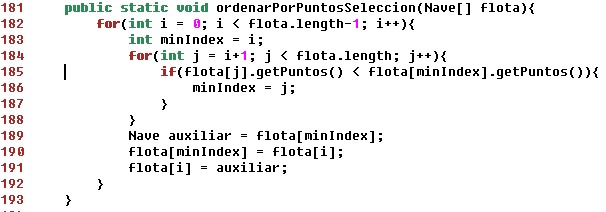
\includegraphics[width=0.9\textwidth,keepaspectratio]{img/9.jpg}
		%\includesvg{img/automata.svg}
		%\label{img:mot2}
		%\caption{Product backlog.}
	\end{figure}
	
	
	\begin{lstlisting}[language=bash,caption={Probando el metodo ordenarPorPuntosSeleccion}][H]	
		javac DemoBatalla.java
		java DemoBatalla
		Nave 1
		Nombre: Hydra
		Fila
		3
		Columna: 4
		Estado: true
		Puntos: 43
		Nave 2
		Nombre: Caza
		Fila
		4
		Columna: 6
		Estado: true
		Puntos: 76
		Nave 3
		Nombre: Misilera
		Fila
		1
		Columna: 6
		Estado: true
		Puntos: 53
		Nave 1: Nombre: Hydra, Fila: 3, Columna: 4, Estado; true, Puntos: 43
		Nave 2: Nombre: Misilera, Fila: 1, Columna: 6, Estado; true, Puntos: 53
		Nave 3: Nombre: Caza, Fila: 4, Columna: 6, Estado; true, Puntos: 76
	\end{lstlisting}
	\begin{lstlisting}[language=bash,caption={Commit: "Metodo ordenarPorPuntosSeleccion culminado" }][H]
		git add DemoBatalla.java
		git commit -m  "Metodo ordenarPorPuntosSeleccion culminado"		
		git push -u origin main
	\end{lstlisting}
	
	
	
	
	
	
	
	\begin{lstlisting}[language=bash,caption={Implementado el método ordenarPorNombreSeleccion }][H]
		vim DemoBatalla.java
	\end{lstlisting}
	
	
	\begin{itemize}	
		\item El método se encarga de hacer un ordenamiento de Strings usando el algoritmo por selección,básicamente la explicación es la misma que se hizo en el método de ordenarPuntosSeleccion , solo que aquí lo única que varía es la condición del if. Como en esta línea se están comparando Strings, se usa el método compareTo, esto con el fin de ordenar de la 'a' hasta la 'z'
	\end{itemize}	
	
	\begin{figure}[H]
		\centering
		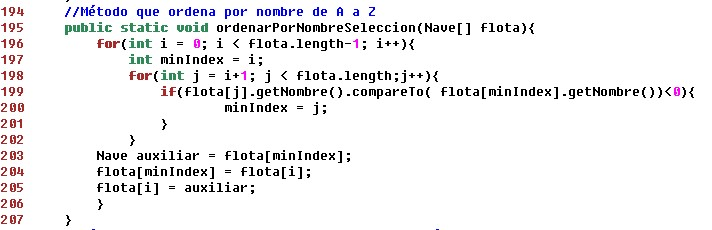
\includegraphics[width=1\textwidth,keepaspectratio]{img/10.jpg}
		%\includesvg{img/automata.svg}
		%\label{img:mot2}
		%\caption{Product backlog.}
	\end{figure}
	
	
	\begin{lstlisting}[language=bash,caption={Probando el metodo ordenarPorNombreSeleccion}][H]	
		javac DemoBatalla.java
		java DemoBatalla
		Nave 1
		Nombre: alfa
		Fila
		3
		Columna: 5
		Estado: true
		Puntos: 56
		Nave 2
		Nombre: xtreme
		Fila
		7
		Columna: 8
		Estado: true
		Puntos: 54
		Nave 3
		Nombre: huascar
		Fila
		3
		Columna: 5
		Estado: true
		Puntos: 87
		Nave 1: Nombre: alfa, Fila: 3, Columna: 5, Estado; true, Puntos: 56
		Nave 2: Nombre: huascar, Fila: 3, Columna: 5, Estado; true, Puntos: 87
		Nave 3: Nombre: xtreme, Fila: 7, Columna: 8, Estado; true, Puntos: 54	
	\end{lstlisting}
	\begin{lstlisting}[language=bash,caption={Commit: "Metodo ordenarPorNombreSeleccion completado" }][H]
		git add DemoBatalla.java
		git commit -m "Metodo ordenarPorNombreSeleccion completado"	
		git push -u origin main
	\end{lstlisting}
	
	
	
	
	\begin{lstlisting}[language=bash,caption={Implementado el método ordenarPorPuntosInsercion }][H]
		vim DemoBatalla.java
	\end{lstlisting}
	
	
	\begin{itemize}	
		\item El método se encarga de hacer un ordenamiento de Puntos usando el algoritmo  de inserción. Básicamente se extrae un elemento de la posición inicial , y se le compara con los elementos de su izquierda, de manera que el lado izquierdo va quedando ordenado 
	\end{itemize}	
	
	\begin{figure}[H]
		\centering
		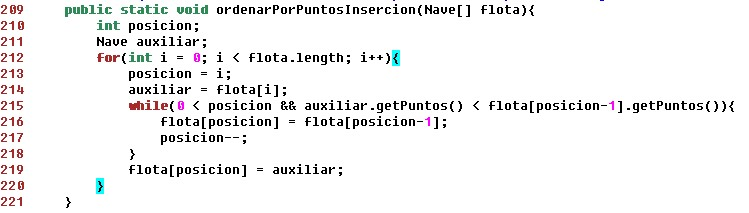
\includegraphics[width=1\textwidth,keepaspectratio]{img/11.jpg}
		%\includesvg{img/automata.svg}
		%\label{img:mot2}
		%\caption{Product backlog.}
	\end{figure}
	
	
	\begin{lstlisting}[language=bash,caption={Probando el metodo ordenarPorPuntoSeleccion}][H]	
		javac DemoBatalla.java
		java DemoBatalla
		Nave 1
		Nombre: epsilon
		Fila
		2
		Columna: 4
		Estado: true
		Puntos: 459
		Nave 2
		Nombre: omega
		Fila
		4
		Columna: 5
		Estado: true
		Puntos: 450
		Nave 3
		Nombre: red
		Fila
		3
		Columna: 7
		Estado: true
		Puntos: 100
		Nave 1: Nombre: red, Fila: 3, Columna: 7, Estado; true, Puntos: 100
		Nave 2: Nombre: omega, Fila: 4, Columna: 5, Estado; true, Puntos: 450
		Nave 3: Nombre: epsilon, Fila: 2, Columna: 4, Estado; true, Puntos: 459
	\end{lstlisting}
	\begin{lstlisting}[language=bash,caption={Commit: "Metodo ordenarPorPuntosInserccion culminado" }][H]
		git add DemoBatalla.java
		git commit -m "Metodo ordenarPorPuntosInserccion culminado"	
		git push -u origin main
	\end{lstlisting}
	
	
	
	
	
	
	
	
	
	
	\begin{lstlisting}[language=bash,caption={Implementado el método ordenarPorNombreInsercion y dándole detalles al código}][H]
		vim DemoBatalla.java
	\end{lstlisting}
	
	
	\begin{itemize}	
		\item El método se encarga de hacer un ordenamiento de Nombres usando el algoritmo  de inserción. Básicamente se extrae un elemento de la posición inicial , y se le compara con los elementos de su izquierda, de manera que el lado izquierdo va quedando ordenado. Se usa compareTo ya que se trata de strings.
	\end{itemize}	
	
	\begin{figure}[H]
		\centering
		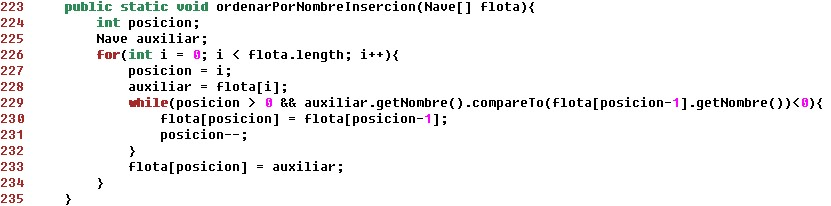
\includegraphics[width=1\textwidth,keepaspectratio]{img/12.jpg}
		%\includesvg{img/automata.svg}
		%\label{img:mot2}
		%\caption{Product backlog.}
	\end{figure}
	
	
	\begin{lstlisting}[language=bash,caption={Probando el metodo ordenarPorNombreInserción}][H]	
		javac DemoBatalla.java
		java DemoBatalla
		Nave 1
		Nombre:
		coraza
		Fila
		4
		Columna: 5
		Estado: true
		Puntos: 5
		Nave 2
		Nombre: venganza
		Fila
		4
		Columna: 6
		Estado: true
		Puntos: 65
		Nave 3
		Nombre: alfa
		Fila
		4
		Columna: 5
		Estado: true
		Puntos: 56
		Nave 4
		Nombre: destructor
		Fila
		4
		Columna: 6
		Estado: true
		Puntos: 32
		Nave 1: Nombre: alfa, Fila: 4, Columna: 5, Estado; true, Puntos: 56
		Nave 2: Nombre: coraza, Fila: 4, Columna: 5, Estado; true, Puntos: 5
		Nave 3: Nombre: destructor, Fila: 4, Columna: 6, Estado; true, Puntos: 32
		Nave 4: Nombre: venganza, Fila: 4, Columna: 6, Estado; true, Puntos: 65
	\end{lstlisting}
	\begin{lstlisting}[language=bash,caption={Commit: "Metodo ordenarPorNombreSelecion culminado" }][H]
		git add DemoBatalla.java
		git commit -m "Metodo ordenarPorNombreSelecion culminado"
		git push -u origin main
	\end{lstlisting}
	
	\begin{itemize}	
		\item * Hubo un error al momento del commit, realmente se está subiendo el método ordenarPorNombreInsercion
	\end{itemize}
	
	
	\begin{lstlisting}[language=bash,caption={Se borran los comenatrios y el numero de elementos del arreglo vuelve a ser de 10 para probarlo}][H]
		vim DemoBatalla.java
	\end{lstlisting}
	
	
	\begin{itemize}	
		\item Ahora lo que se hace para un mejor seguimiento de la ejecución del código es aumentar líneas que imprimen un mensaje el cual indica lo que se está mostrando.
	\end{itemize}
	
	\begin{lstlisting}[language=bash,caption={Probando DemoBatalla.java }][H]	
		javac DemoBatalla.java
		java DemoBatalla
	    Nave 1
	    Nombre: coraza
	    Fila
	    3
	    Columna: 4
	    Estado: true
	    Puntos: 54
	    Nave 2
	    Nombre: alcon
	    Fila
	    4
	    Columna: 7
	    Estado: true
	    Puntos: 43
	    Nave 3
	    Nombre: venganza
	    Fila
	    2
	    Columna: 4
	    Estado: false
	    Puntos: 32
	    Nave 4
	    Nombre: huascar
	    Fila
	    2
	    Columna: 9
	    Estado: true
	    Puntos: 80
	    Nave 5
	    Nombre: peregrino
	    Fila
	    1
	    Columna: 7
	    Estado: true
	    Puntos: 49
	    Nave 6
	    Nombre: alfa
	    Fila
	    2
	    Columna: 5
	    Estado: true
	    Puntos: 15
	    Nave 7
	    Nombre: alcon
	    Fila
	    4
	    Columna: 7
	    Estado: true
	    Puntos: 53
	    Nave 8
	    Nombre: milenario
	    Fila
	    8
	    Columna: 4
	    Estado: false
	    Puntos: 30
	    Nave 9
	    Nombre: destructor
	    Fila
	    3
	    Columna: 6
	    Estado: true
	    Puntos: 47
	    Nave 10
	    Nombre: omega
	    Fila
	    2
	    Columna: 3
	    Estado: false
	    Puntos: 56
	    
	    Naves creadas:
	    Nave 1: Nombre: coraza, Fila: 3, Columna: 4, Estado; true, Puntos: 54
	    Nave 2: Nombre: alcon, Fila: 4, Columna: 7, Estado; true, Puntos: 43
	    Nave 3: Nombre: venganza, Fila: 2, Columna: 4, Estado; false, Puntos: 32
	    Nave 4: Nombre: huascar, Fila: 2, Columna: 9, Estado; true, Puntos: 80
	    Nave 5: Nombre: peregrino, Fila: 1, Columna: 7, Estado; true, Puntos: 49
	    Nave 6: Nombre: alfa, Fila: 2, Columna: 5, Estado; true, Puntos: 15
	    Nave 7: Nombre: alcon, Fila: 4, Columna: 7, Estado; true, Puntos: 53
	    Nave 8: Nombre: milenario, Fila: 8, Columna: 4, Estado; false, Puntos: 30
	    Nave 9: Nombre: destructor, Fila: 3, Columna: 6, Estado; true, Puntos: 47
	    Nave 10: Nombre: omega, Fila: 2, Columna: 3, Estado; false, Puntos: 56
	    Ingrese el nombre de la nave que desea buscar
	    huascar
	    Nombre: huascar, Fila: 2, Columna: 9, Estado; true, Puntos: 80
	    Ingrese los puntos para hacer la busqueda de resultados menores o igual
	    33
	    Nombre: venganza, Fila: 2, Columna: 4, Estado; false, Puntos: 32
	    Nombre: alfa, Fila: 2, Columna: 5, Estado; true, Puntos: 15
	    Nombre: milenario, Fila: 8, Columna: 4, Estado; false, Puntos: 30
	    
	    
	    Nave con mayor numero de puntos: Nombre: huascar, Fila: 2, Columna: 9, Estado; true, Puntos: 80
	    Se usara busqueda lineal para encontrar el nombre solicitado
	    Ingrese algun nombre de una nave
	    alcon
	    Nave encontrada Nombre: alcon, Fila: 4, Columna: 7, Estado; true, Puntos: 43
	    Se usara ordenamiento burbuja para ordenar los puntos
	    Nave 1: Nombre: alfa, Fila: 2, Columna: 5, Estado; true, Puntos: 15
	    Nave 2: Nombre: milenario, Fila: 8, Columna: 4, Estado; false, Puntos: 30
	    Nave 3: Nombre: venganza, Fila: 2, Columna: 4, Estado; false, Puntos: 32
	    Nave 4: Nombre: alcon, Fila: 4, Columna: 7, Estado; true, Puntos: 43
	    Nave 5: Nombre: destructor, Fila: 3, Columna: 6, Estado; true, Puntos: 47
	    Nave 6: Nombre: peregrino, Fila: 1, Columna: 7, Estado; true, Puntos: 49
	    Nave 7: Nombre: alcon, Fila: 4, Columna: 7, Estado; true, Puntos: 53
	    Nave 8: Nombre: coraza, Fila: 3, Columna: 4, Estado; true, Puntos: 54
	    Nave 9: Nombre: omega, Fila: 2, Columna: 3, Estado; false, Puntos: 56
	    Nave 10: Nombre: huascar, Fila: 2, Columna: 9, Estado; true, Puntos: 80
	    Se usara ordenamiento burbuja para ordenar los nombres
	    Nave 1: Nombre: alcon, Fila: 4, Columna: 7, Estado; true, Puntos: 43
	    Nave 2: Nombre: alcon, Fila: 4, Columna: 7, Estado; true, Puntos: 53
	    Nave 3: Nombre: alfa, Fila: 2, Columna: 5, Estado; true, Puntos: 15
	    Nave 4: Nombre: coraza, Fila: 3, Columna: 4, Estado; true, Puntos: 54
	    Nave 5: Nombre: destructor, Fila: 3, Columna: 6, Estado; true, Puntos: 47
	    Nave 6: Nombre: huascar, Fila: 2, Columna: 9, Estado; true, Puntos: 80
	    Nave 7: Nombre: milenario, Fila: 8, Columna: 4, Estado; false, Puntos: 30
	    Nave 8: Nombre: omega, Fila: 2, Columna: 3, Estado; false, Puntos: 56
	    Nave 9: Nombre: peregrino, Fila: 1, Columna: 7, Estado; true, Puntos: 49
	    Nave 10: Nombre: venganza, Fila: 2, Columna: 4, Estado; false, Puntos: 32
	    Se usara busqueda binaria para encontrar el nombre de la nave a buscar
	    Ingrese la nave que desea buscar
	    utopia
	    Nave no encontrada
	    Se empleara orden por seleccion en los puntos
	    Nave 1: Nombre: alfa, Fila: 2, Columna: 5, Estado; true, Puntos: 15
	    Nave 2: Nombre: milenario, Fila: 8, Columna: 4, Estado; false, Puntos: 30
	    Nave 3: Nombre: venganza, Fila: 2, Columna: 4, Estado; false, Puntos: 32
	    Nave 4: Nombre: alcon, Fila: 4, Columna: 7, Estado; true, Puntos: 43
	    Nave 5: Nombre: destructor, Fila: 3, Columna: 6, Estado; true, Puntos: 47
	    Nave 6: Nombre: peregrino, Fila: 1, Columna: 7, Estado; true, Puntos: 49
	    Nave 7: Nombre: alcon, Fila: 4, Columna: 7, Estado; true, Puntos: 53
	    Nave 8: Nombre: coraza, Fila: 3, Columna: 4, Estado; true, Puntos: 54
	    Nave 9: Nombre: omega, Fila: 2, Columna: 3, Estado; false, Puntos: 56
	    Nave 10: Nombre: huascar, Fila: 2, Columna: 9, Estado; true, Puntos: 80
	    Se empleara orden por insercion en los puntos
	    Nave 1: Nombre: alfa, Fila: 2, Columna: 5, Estado; true, Puntos: 15
	    Nave 2: Nombre: milenario, Fila: 8, Columna: 4, Estado; false, Puntos: 30
	    Nave 3: Nombre: venganza, Fila: 2, Columna: 4, Estado; false, Puntos: 32
	    Nave 4: Nombre: alcon, Fila: 4, Columna: 7, Estado; true, Puntos: 43
	    Nave 5: Nombre: destructor, Fila: 3, Columna: 6, Estado; true, Puntos: 47
	    Nave 6: Nombre: peregrino, Fila: 1, Columna: 7, Estado; true, Puntos: 49
	    Nave 7: Nombre: alcon, Fila: 4, Columna: 7, Estado; true, Puntos: 53
	    Nave 8: Nombre: coraza, Fila: 3, Columna: 4, Estado; true, Puntos: 54
	    Nave 9: Nombre: omega, Fila: 2, Columna: 3, Estado; false, Puntos: 56
	    Nave 10: Nombre: huascar, Fila: 2, Columna: 9, Estado; true, Puntos: 80
	    Se empleara orden por seleccion en los nombres
	    Nave 1: Nombre: alcon, Fila: 4, Columna: 7, Estado; true, Puntos: 43
	    Nave 2: Nombre: alcon, Fila: 4, Columna: 7, Estado; true, Puntos: 53
	    Nave 3: Nombre: alfa, Fila: 2, Columna: 5, Estado; true, Puntos: 15
	    Nave 4: Nombre: coraza, Fila: 3, Columna: 4, Estado; true, Puntos: 54
	    Nave 5: Nombre: destructor, Fila: 3, Columna: 6, Estado; true, Puntos: 47
	    Nave 6: Nombre: huascar, Fila: 2, Columna: 9, Estado; true, Puntos: 80
	    Nave 7: Nombre: milenario, Fila: 8, Columna: 4, Estado; false, Puntos: 30
	    Nave 8: Nombre: omega, Fila: 2, Columna: 3, Estado; false, Puntos: 56
	    Nave 9: Nombre: peregrino, Fila: 1, Columna: 7, Estado; true, Puntos: 49
	    Nave 10: Nombre: venganza, Fila: 2, Columna: 4, Estado; false, Puntos: 32
	    Se empleara orden por insercion en los nombres
	    Nave 1: Nombre: alcon, Fila: 4, Columna: 7, Estado; true, Puntos: 43
	    Nave 2: Nombre: alcon, Fila: 4, Columna: 7, Estado; true, Puntos: 53
	    Nave 3: Nombre: alfa, Fila: 2, Columna: 5, Estado; true, Puntos: 15
	    Nave 4: Nombre: coraza, Fila: 3, Columna: 4, Estado; true, Puntos: 54
	    Nave 5: Nombre: destructor, Fila: 3, Columna: 6, Estado; true, Puntos: 47
	    Nave 6: Nombre: huascar, Fila: 2, Columna: 9, Estado; true, Puntos: 80
	    Nave 7: Nombre: milenario, Fila: 8, Columna: 4, Estado; false, Puntos: 30
	    Nave 8: Nombre: omega, Fila: 2, Columna: 3, Estado; false, Puntos: 56
	    Nave 9: Nombre: peregrino, Fila: 1, Columna: 7, Estado; true, Puntos: 49
	    Nave 10: Nombre: venganza, Fila: 2, Columna: 4, Estado; false, Puntos: 32
	\end{lstlisting}
	
	\begin{lstlisting}[language=bash,caption={Commit: "Subiendo DemoBatalla.java del lab04 en su version terminada" }][H]
		git add DemoBatalla.java
		git commit -m "Subiendo DemoBatalla.java del lab04 en su version terminada"
		git push -u origin main
	\end{lstlisting}
	
	
		\subsection{Estructura de laboratorio 01}
	\begin{itemize}	
		\item El contenido que se entrega en este laboratorio es el siguiente:
	\end{itemize}
	
	\begin{lstlisting}[style=ascii-tree]
		lab04
		|   DemoBatalla.java
		|   Nave.java
		|
		|──latex
		|      programacion_lab04_rescobedoq_v1.0.pdf
		|      programacion_lab04_rescobedoq_v1.0.tex
		|     
		|	    img
		|       	   1.jpg
		|        	10.jpg
		|        	11.jpg
		|        	12.jpg
		|        	2.jpg
		|        	3.jpg
		|		     	4.jpg	
		|       	   5.jpg
		|       	   6.jpg
		|       	   7.jpg
		|       	   8.jpg
		|       	   9.jpg
		|       	   logo_abet.png
		|       	   logo_episunsa.png
		|      		logo_unsa.jpg
		|
				src
	\end{lstlisting} 
	
	
	
	
	
	
	\section{\textcolor{red}{Rúbricas}}
	
	\subsection{\textcolor{red}{Entregable Informe}}
	\begin{table}[H]
		\caption{Tipo de Informe}
		\setlength{\tabcolsep}{0.5em} % for the horizontal padding
		{\renewcommand{\arraystretch}{1.5}% for the vertical padding
			\begin{tabular}{|p{3cm}|p{12cm}|}
				\hline
				\multicolumn{2}{|c|}{\textbf{\textcolor{red}{Informe}}}  \\
				\hline 
				\textbf{\textcolor{red}{Latex}} & \textcolor{blue}{El informe está en formato PDF desde Latex,  con un formato limpio (buena presentación) y facil de leer.}   \\ 
				\hline 
				
				
			\end{tabular}
		}
	\end{table}
	
	\clearpage
	
	\subsection{\textcolor{red}{Rúbrica para el contenido del Informe y demostración}}
	\begin{itemize}			
		\item El alumno debe marcar o dejar en blanco en celdas de la columna \textbf{Checklist} si cumplio con el ítem correspondiente.
		\item Si un alumno supera la fecha de entrega,  su calificación será sobre la nota mínima aprobada, siempre y cuando cumpla con todos lo items.
		\item El alumno debe autocalificarse en la columna \textbf{Estudiante} de acuerdo a la siguiente tabla:
		
		\begin{table}[ht]
			\caption{Niveles de desempeño}
			\begin{center}
				\begin{tabular}{ccccc}
					\hline
					& \multicolumn{4}{c}{Nivel}\\
					\cline{1-5}
					\textbf{Puntos} & Insatisfactorio 25\%& En Proceso 50\% & Satisfactorio 75\% & Sobresaliente 100\%\\
					\textbf{2.0}&0.5&1.0&1.5&2.0\\
					\textbf{4.0}&1.0&2.0&3.0&4.0\\
					\hline
				\end{tabular}
			\end{center}
		\end{table}	
		
	\end{itemize}
	
	\begin{table}[H]
		\caption{Rúbrica para contenido del Informe y demostración}
		\setlength{\tabcolsep}{0.5em} % for the horizontal padding
		{\renewcommand{\arraystretch}{1.5}% for the vertical padding
			%\begin{center}
			\begin{tabular}{|p{2.7cm}|p{7cm}|x{1.3cm}|p{1.2cm}|p{1.5cm}|p{1.1cm}|}
				\hline
				\multicolumn{2}{|c|}{Contenido y demostración} & Puntos & Checklist & Estudiante & Profesor\\
				\hline
				\textbf{1. GitHub} & Hay enlace URL activo del directorio para el  laboratorio hacia su repositorio GitHub con código fuente terminado y fácil de revisar. &2 &X &2 & \\ 
				\hline
				\textbf{2. Commits} &  Hay capturas de pantalla de los commits más importantes con sus explicaciones detalladas. (El profesor puede preguntar para refrendar calificación). &4 &X &2 & \\ 
				\hline 
				\textbf{3. Código fuente} &  Hay porciones de código fuente importantes con numeración y explicaciones detalladas de sus funciones. &2 &X &2 & \\ 
				\hline 
				\textbf{4. Ejecución} & Se incluyen ejecuciones/pruebas del código fuente  explicadas gradualmente. &2 &X &1 & \\ 
				\hline			
				\textbf{5. Pregunta} & Se responde con completitud a la pregunta formulada en la tarea.  (El profesor puede preguntar para refrendar calificación).  &2 &X &2 & \\ 
				\hline	
				\textbf{6. Fechas} & Las fechas de modificación del código fuente estan dentro de los plazos de fecha de entrega establecidos. &2 &X &2 & \\ 
				\hline 
				\textbf{7. Ortografía} & El documento no muestra errores ortográficos. &2 &X &1 & \\ 
				\hline 
				\textbf{8. Madurez} & El Informe muestra de manera general una evolución de la madurez del código fuente,  explicaciones puntuales pero precisas y un acabado impecable.   (El profesor puede preguntar para refrendar calificación).  &4 &X &4 & \\ 
				\hline
				\multicolumn{2}{|c|}{\textbf{Total}} &20 & &16 & \\ 
				\hline
			\end{tabular}
			%\end{center}
			%\label{tab:multicol}
		}
	\end{table}
	
	\clearpage
	
	\section{Referencias}
	\begin{itemize}			
		\item \url{https://drive.google.com/file/d/1CoQAKeKW-QDYRmHLrBdbSopFB1Z_Qmk3/view?usp=drive_link}
	\end{itemize}	
	
	%\clearpage
	%\bibliographystyle{apalike}
	%\bibliographystyle{IEEEtranN}
	%\bibliography{bibliography}
	
\end{document}